\chapter{相关工作}
\label{cha:china}
本章首先介绍Mesh网络架构,对现有的工业界和学术界的Mesh网络实验平台和项目做综述,
然后总结它们的贡献、优势和缺陷。然后介绍QoS在802.11协议族中的基本实现机制,并讨
论在Mesh网络中应用QoS保障面临的困难。最后集中在Mesh网络基础上的视频传输QoS保障
技术的研究应用。

\section{无线Mesh网络}
在存在基础管理结构的无线网络中,路由信息通常由中央控制的角色提供,如AP网络中的AC。
这样可以实现网络资源的全局调度和管控。相反,在ad-hoc模式下,不存在中央控制的角色,
网络中的路由构建由参与网络的节电设备自发交互完成。作为典型的ad-hoc模式的无线网络
架构,无线Mesh网络中的节点之间通过交互链路状态和局部路由信息从而构建起全局的网状
网络架构。

无线Mesh网络由Mesh路由器,Mesh客户端组成。其中,Mesh路由器提供路由构建和异构网络
接入的功能。Mesh客户端为用户接入Mesh网络提供接口。[插图]

无线Mesh网络是具有广阔应用前景的下一代无线网络技术。其自组织、移动和灵活的网络构
建使其能够适用于很多传统网络无法覆盖的场景,比如:救灾、野外、战场等临时性应用且
缺乏有线网络基础设施,并且可以作为3G/4G网络的一个很好的延伸。无线Mesh网络的主要
优势体现在快速、低成本的部署和大范围的网络覆盖。

在过去的十多年里,伴随着无线Mesh网络的研究热潮,很多的项目开发了不同的Mesh网络路
由协议,802.11协议簇也将Mesh网络的标准制定纳入讨论并以提出完善的修正案。但目前80
2.11所提出的修正案中的Mesh路由协议并没有在工业界得到广泛的使用,各种不同的路由协
议仍然以各自的社区为依托不断发展完善。

\section{无线Mesh网络中的路由技术}
在无线mesh网络中,当节点互相不在信号覆盖范围内时,就需要中继节点代为转发。很多的
Mesh网络协议可以完成这一功能,本节就描述其中一些典型的协议以及它们之间的差异。

无线Mesh网络通常采用分布式路由,即网络中的节点分发并采集其他节点的局部路由信息。
然后,每个节点根据收集到的网络路由信息,决定到达目的节点的最佳路径。分布式路由协
议又可以分为主动式和反应式两种不同的类别。主动式路由协议中,节点周期性的广播自己
的存在,并携带自己所知道的局部路由信息;反应式路由协议则在需要发送数据的时候,即
时获取路由信息。Mesh网络的架构和无线介质的特殊性给路由构建带来了一些特殊的挑战。

\begin{itemize}
  \item[-] 竞争使用共享的无线信道会限制网络的性能。
  \item[-] 用于网络构建的数据包造成额外的开销。
  \item[-] 需要引入漫游机制解决移动节点的接入问题。
  \item[-] 当网络中一个节点失效,可能导致多条路由瞬间失效。
\end{itemize}

各种不同的协议采用不同的方式解决这些问题,但殊途同归,最终的目标都是最小化网络构
建的额外开销,同时保证最大化网络吞吐量、网络的性能,并保持连接的有效性。

\subsection{主要路由技术}
如前所述,Mesh网络中的路由技术可以分为主动式路由和反应式路由。如果路由信息的收集
和路由的计算在节点需要发送数据时才进行,则该路由方式成为反应式路由。反之,如果网
络的信息分布式存储在网络中的节点中,且每当网络中的状态发生变化,该变化会即时广播
全网络,相关的节点即时更新自己的路由信息,这种路由方式称为主动式路由。

大多数Mesh路由协议收集信息和判定路由时以如下两种方式为主要的判定依据:链路状态和
距离向量。

基于链路状态的路由,节点将自己相邻链路信息组织成有向图的形式,洪泛全网。每个节点
可以收集到其他节点的局部链路拓扑和质量信息,并基于此构建整个网络的拓扑信息,并基
于不同拓扑路由的权重计算出最短路径,即发送数据时的路由。

基于距离向量的路由,节点仅知道目标节点数据需要送达的下一跳节点,即数据发送的方向。
而最佳的下一跳节点的选择则基于到达目标节点的总跳数和每一跳的链路质量。距离向量路
由方式不需要计算完整的网络拓扑,因此消耗的额外开销更少。缺点是,得到的路由通常不
是全局最优的。

分布式路由需要处理网络中的路由环路现象。路由环路通常出现在两个或者更多的节点之间,
路由环路会导致数据陷入环路,造成额外的网络开销,且数据始终无法送达最终的目的节点。

\subsection{优化的链路状态路由(OLSR)}
优化的链路状态路由(OLSR)广泛的应用于基于嵌入式Linux平台的Mesh网络中。通常作为守
护进程运行在网络层,属于主动式路由,且基于链路状态做路由决策。

在最初的OLSR实现中,网络拓扑图的计算很慢且经常在网络状态发生更新的时失效。路由变
化频繁,易形成路由环路,造成网络的低可用性。为了解决这些问题,OLSR引入了信的路由
决策参数--传输次数期望(ETX)。新的参数带来了性能的显著提升,但仍然没有解决路由
环路的问题。通过增加拓扑控制数据包的发送频率可以一定程度上降低路由环路的形成次数。
由此造成的额外的路由开销可以通过限制洪泛距离予以限制--仅向三跳之内的邻居节点洪
泛路由变化信息,这种方法在实践中被证明是有效的。这种技术称为鱼眼机制(Fish Eye),
该技术保证了OLSR的可用性,尽管路由环路还是会偶尔出现。

\subsection{Ad-hoc网络需求驱动的距离向量路由协议(AODV)}
Ad-hoc网路需求驱动的距离向量路由协议(AODV)是一种基于距离向量的反应式路由协议。
在该路由协议中,当有节点需要发送数据到目的节点,就先向网络广播路由请求数据包,通
过网络中其他节点包括目的节点的相应,构建瞬时的有效路由。当网络处于相对空闲状态时,
该协议最大程度上减少了额外的路由开销。该协议在对能耗要求极高的传感器网络中具有很
好的应用价值。

\subsection{针对移动Ad-hoc网络的路由协议(BATMAN)}
针对移动Ad-hoc网络的路由协议2006年诞生,最初最为OLSR的替代者,属于基于距离向量的
主动路由协议。在最初的三个版本中,BATMAN引入了许多特性,包括:不对称链路,多接口
支持等。类似于OSLR,该协议同样作为用户层的守护进程运行再路由层。

\subsection{BATMAN升级版(BATMAN-adv)}
因为BATMAN运行再用户层所带来的性能问题,BATMAN-adv再2007年开始投入研发。因为运行
再内核态,新的协议节省了大量的内核态和用户态之间拷贝数据包的开销。另一方面,新的
协议运行再链路层,用mac地址做路由。

BATMAN-adv在链路层对数据做封装,对网络层透明,因此可以兼容其他的网络层协议,也使
得其他特性得加入更加容易。现在得BATMAN-adv支持非Mesh设备得桥接和漫游。

2011年,BATMAN-adv已经添加进Linux内核开发主线树。

\section{802.11协议簇QoS支持}
802.11标准族有对无线网络的QoS保障的标准--802.11e。802.11e将mac层数据按照数据的
业务类型划分为四个不同的优先级队列,每一个队列在竞争使用无线信道是具有不同的优先
级,优先级通过竞争窗口大小的设置从而控制竞争成功的概率实现。

\section{无线Mesh网络视频传输}
本文的主要工作为基于无线Mesh网络搭建高性能实时视频流传输系统。该领域已经有过诸多
的探索性工作,本节对相关工作做总结归纳。

工作一[real-time video surveillance over IEEE802.11 Mesh Network]中,作者提出在
视频流应用的场景中,为了在摄像头数量增多时最大限度的保证图像质量,需要提升网络的
高可用性。实验发现,使用标准802.11 DCF MAC协议通讯,当每个摄像头的视频流占用带宽
在1Mbps时,系统最大可负载的摄像头数量大约为5-6个。当摄像头超过这个数量时,就会出
现严重的抖动现象从而影响视频质量。文章认为性能的显著下降来自于多跳场景下隐终端的
影响。针对这一问题,文章提出了一种时间同步的应用层MAC协议-TSAM,该协议运行在802.11
之上。TSAM禁用了802.11的冲突退避机制,并基于时分复用技术给每一个节点分配时间窗口,
从而消除了竞争,保证无线信道的最大可用性。实验显示,TSAM在控制端到端延时的同时通
过顺序时间窗口保证了节点之间的同步。

该工作对节点设备的时钟同步要求较高,且需要修改现有802.11协议的冲突退避机制,不能
够很好的兼容协议。

工作二[Video-aware Multicast Opportunistic Routing over 802.11 two-hop mesh networks]
提出并特征化了一种针对视频流多播的机会路由算法,该算法特别适用于两跳之内的无线Mesh
网络。文章通过分类不同的视频数据并赋予不同的权重,从而提升QoS。对于视频流数据而言,
延时是一个重要的考量的指标,相比之下,即使因此发生一定的丢包都可以接受。基于此,文
章提出ViMOR,一种视频流多播机会路由协议,且聚焦于跳数小于等于两跳的拓扑结构。相比
于MORE,ViMOR能够提升网络的吞吐量同时提升视频接受的质量。

工作三[Video Multicast over Wireless Mesh Networks with Scalable Video Coding (SVC)]
中,作者提出了一种挑选对等节点的参数-MSM(Multiplication Selector Metric)。该参
数可以解决传统的基于假发的参数面临的两个局限:瓶颈链路的识别和跳数计数。再此基础
上,文章提出了一种基于无线链路质量感知的对等节点选择机制-WLO(Wireless Link quality-
aware Overlay)。WLO根据MSM参数的值在存有目标内容的对等网络节点中选择最优的节点。






\section{其它例子}
\label{sec:other}

在第~\ref{cha:intro} 章中我们学习了贝叶斯公式~(\ref{equ:chap1:bayes}),这里我们复
习一下:
\begin{equation}
\label{equ:chap2:bayes}
p(y|\mathbf{x}) = \frac{p(\mathbf{x},y)}{p(\mathbf{x})}=
\frac{p(\mathbf{x}|y)p(y)}{p(\mathbf{x})}
\end{equation}

\subsection{绘图}
\label{sec:draw}

本模板不再预先装载任何绘图包(如 \pkg{pstricks,pgf} 等),完全由用户来决定。
个人觉得 \pkg{pgf} 不错,不依赖于 Postscript。此外还有很多针对 \LaTeX{} 的
 GUI 作图工具,如 XFig(jFig), WinFig, Tpx, Ipe, Dia, Inkscape, LaTeXPiX,
jPicEdt, jaxdraw 等等。

\subsection{插图}
\label{sec:graphs}

强烈推荐《\LaTeXe\ 插图指南》!关于子图形的使用细节请参看 \pkg{subcaption} 宏包的说明文档。

\subsubsection{一个图形}
\label{sec:onefig}
一般图形都是处在浮动环境中。之所以称为浮动是指最终排版效果图形的位置不一定与源文
件中的位置对应\footnote{This is not a bug, but a feature of \LaTeX!},这也是刚使
用 \LaTeX{} 同学可能遇到的问题。如果要强制固定浮动图形的位置,请使用 \pkg{float} 宏包,
它提供了 \texttt{[H]} 参数,比如图~\ref{fig:xfig1}。
\begin{figure}[H] % use float package if you want it here
  \centering
  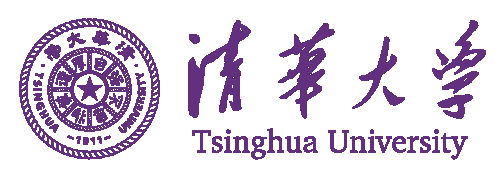
\includegraphics{thu-whole-logo}
  \caption{利用 Xfig 制图}
  \label{fig:xfig1}
\end{figure}

大学之道,在明明德,在亲民,在止于至善。知止而后有定;定而后能静;静而后能安;安
而后能虑;虑而后能得。物有本末,事有终始。知所先后,则近道矣。古之欲明明德于天
下者,先治其国;欲治其国者,先齐其家;欲齐其家者,先修其身;欲修其身者,先正其心;
欲正其心者,先诚其意;欲诚其意者,先致其知;致知在格物。物格而后知至;知至而后
意诚;意诚而后心正;心正而后身 修;身修而后家齐;家齐而后国治;国治而后天下
平。自天子以至于庶人,壹是皆以修身为本。其本乱而未治者 否矣。其所厚者薄,而其所
薄者厚,未之有也!

\hfill —— 《大学》


\subsubsection{多个图形}
\label{sec:multifig}

如果多个图形相互独立,并不共用一个图形计数器,那么
用 \texttt{minipage} 或者\texttt{parbox} 就可以。否则,请参看
图~\ref{fig:big1-subcaptionbox},它包含两个小图,分别是图~\ref{fig:subfig1}和
图~\ref{fig:subfig2}。推荐使用\cs{subcaptionbox},因为可以像
图~\ref{fig:big1-subcaptionbox} 那样对齐子图的标题,也可以使
用\pkg{subcaption}宏包的\cs{subcaption}(放在 minipage中,用法同\cs{caption})
或是 \pkg{subfigure} 、 \pkg{subtable}环境,像图~\ref{fig:big1-subfigure},
不要再用 \cs{subfloat}、\cs{subfigure} 和 \cs{subtable}。

\begin{figure}[h]
  \centering%
  \subcaptionbox{第一个小图形\label{fig:subfig1}}[3cm] %标题的长度,超过则会换行,如下一个小图。
    {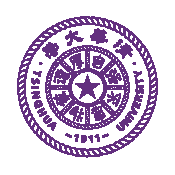
\includegraphics[height=3cm]{thu-fig-logo}}%
  \hspace{4em}%
  \subcaptionbox{第二个小图形,注意这个图略矮些。如果标题很长的话,它会自动换行\label{fig:subfig2}}
      {
\includegraphics[height=2cm]{thu-text-logo}}
  \caption{包含子图形的大图形(subcaptionbox示例)}
  \label{fig:big1-subcaptionbox}
\end{figure}
\begin{figure}[h]
  \centering%
  \begin{subfigure}{3cm}
    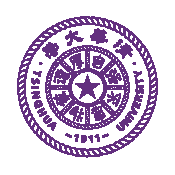
\includegraphics[height=3cm]{thu-fig-logo}
    \caption{第一个小图形}
  \end{subfigure}%
  \hspace{4em}%
  \begin{subfigure}{0.5\textwidth}
    
\includegraphics[height=2cm]{thu-text-logo}
    \caption{第二个小图形,注意这个图略矮些。subfigure中同一行的子图在顶端对齐。}
  \end{subfigure}
  \caption{包含子图形的大图形(subfigure示例)}
  \label{fig:big1-subfigure}
\end{figure}

古之学者必有师。师者,所以传道受业解惑也。人非生而知之者,孰能无惑?惑而不从师,
其为惑也,终不解矣。生乎吾前,其闻道也固先乎吾,吾从而师之;生乎吾後,其闻道也亦
先乎吾,吾从而师之。吾师道也,夫庸知其年之先後生於吾乎!是故无贵无贱无长无少,道
之所存,师之所存也。

嗟乎!师道之不传也久矣,欲人之无惑也难矣。古之圣人,其出人也远矣,犹且从师而问焉;
今之众人,其下圣人也亦远矣,而耻学於师。是故圣益圣,愚益愚。圣人之所以为圣,愚
人之所以为愚,其皆出於此乎?爱其子,择师而教之,於其身也,则耻师焉,惑焉。彼童子
之师,授之书而习其句读者,非吾所谓传其道、解其惑者也。句读之不知,惑之不解,或师
焉,或不焉,小学而大遗,吾未见其明也。巫医、乐师、百工之人不耻相师,  士大夫之族
曰“师”曰“弟子”之云者,则群聚而笑之。问之,则曰:彼与彼年相若也,道相似也,位
卑则足羞,官盛则近谀。呜呼!师道之不复,可知矣。巫医、乐师、百工之人。吾子不齿,
今其智乃反不能及,其可怪也欤!圣人无常师。孔子师郯子、苌子、师襄、老聃。郯子之徒,
其贤不及孔子。孔子曰:“三人行,必有我师。”是故弟子不必不如师,师不必贤於弟子。
闻道有先後,术业有专攻,如是而已。

如果要把编号的两个图形并排,那么小页就非常有用了:
\begin{figure}
\begin{minipage}{0.48\textwidth}
  \centering
  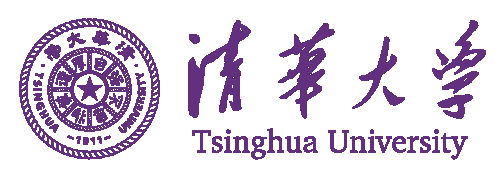
\includegraphics[height=2cm]{thu-whole-logo}
  \caption{并排第一个图}
  \label{fig:parallel1}
\end{minipage}\hfill
\begin{minipage}{0.48\textwidth}
  \centering
  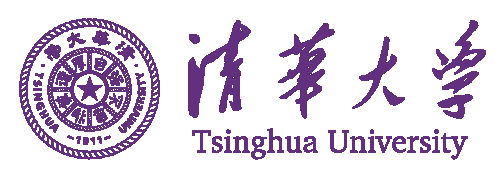
\includegraphics[height=2cm]{thu-whole-logo}
  \caption{并排第二个图}
  \label{fig:parallel2}
\end{minipage}
\end{figure}

李氏子蟠,年十七,好古文、六艺,经传皆通习之,不拘於时,学於余。余嘉其能行古
道,作师说以贻之。

\hfill —— 韩愈(唐)
